\chapter{Reproducibility}
\label{sec:repro}

\makeatletter
\@ifundefined{promptinline}{%
  \newcommand{\promptinline}[1]{\mbox{\normalfont\footnotesize\sffamily\(\langle\)\,#1\,\(\rangle\)}}%
}{%
  \renewcommand{\promptinline}[1]{\mbox{\normalfont\footnotesize\sffamily\(\langle\)\,#1\,\(\rangle\)}}%
}
\makeatother

\section{Two-Digit Addition Circuit Reproduction in Qwen3-4B}

\citet{lindsey2025biology} report that Claude~3.5 Haiku does not solve
prompts of the form \promptinline{calc:~a+b=} by a symbolic carry
algorithm.  The reported circuit instead uses sparse lookup features localised
by the ones digits of the two operands.  A feature may activate when
$a \bmod 10 = d_1$ and $b \bmod 10 = d_2$, then route the ones digit of
$d_1+d_2$ toward the output.  We use this result as the hypothesis for Qwen3-4B.  The
prior work gives the target pattern, but not every implementation detail needed
for this model.  We therefore state our Qwen procedure explicitly, using the
transcoder notation of Section~\ref{sec:interp-methods}.

\subsection{Operand and Residue Feature Scan}
\label{subsec:operand-plots}

For a prompt \promptinline{calc:~a + b =~}, let $T$ be the index of the
\promptinline{=} token.  For each feature $(\ell,k)$, we define the operand
matrix

\begin{equation}
  M_{\ell,k}[a,b]
    \;=\; a_{\ell,k,T}
          \left( \text{\promptinline{calc:~a + b =~}}\right),
    \qquad a,b \in \{0,\ldots,99\}.
  \label{eq:operand-matrix}
\end{equation}

This matrix turns feature activation into geometry, raw-sum features form
diagonals, and single-operand features form horizontal or vertical bands.
Also, ones-digit features repeat every ten cells and joint lookup features form regular
grids of point clusters.  We grade candidate lookup features with the
concentration score

\begin{equation}
  s_{\ell,k}(d_1,d_2)
    \;=\;
    \frac{%
      \displaystyle\sum_{a,b}
        M_{\ell,k}[a,b]\;
        \mathbb{1}\!\left[
          a \bmod 10 \in \{d_1,d_2\},\;
          b \bmod 10 \in \{d_1,d_2\}
        \right]
    }{%
      \displaystyle\sum_{a,b} M_{\ell,k}[a,b]
    }.
  \label{eq:lookup-score}
\end{equation}

We discard features with very small peak activation ($a_{\ell,k,T} \leq10^{-5}$), then rank the rest by
$s_{\ell,k}$.  For the focus prompt \promptinline{calc:~36+59=}, we take the
top-ranked feature for the digit pair $(6,9)$ as the reference lookup feature.
We then run two causal checks.  In the inhibition check, we scale its activation
by $\beta \in \{1.0,0.5,0.0,-1.0,-5.0,-10.0\}$.  If the feature is necessary,
lower $\beta$ should reduce support for the correct ones digit.  In the
substitution check, we replace earlier MLP inputs by those from
\promptinline{calc:~39+59=}.  If the feature mediates the computation, the
represented ones digit should shift from $5$ to $8$.

\paragraph{Token-position feature localisation.}
\citet{lindsey2025biology} report that operand-token features encode individual
digits, while delimiter-token features encode digit combinations.  We test this
separation in Qwen3-4B by applying Equation~\ref{eq:operand-matrix} at the ones
digit of $a$, position $4$, the ones digit of $b$, position $7$, and the
\promptinline{=} token, position $8$.  At each position, we select the top $15$
CLT features by attribution edge weight and retain one representative for each
distinct ones digit.  Figure~\ref{fig:operand-pos-scan} shows the scan.

At position $4$, features form vertical period-10 bands and encode
$a \bmod 10$ with little dependence on $b$.  At position $7$, features form the
transposed pattern and encode $b \bmod 10$ with little dependence on $a$.  At
the \promptinline{=} token, the two streams meet.  Some features form diagonals
of constant $a+b$.  Others form point-cluster grids selective to pairs of ones
digits.  The circuit therefore separates the two digits first, then combines the
two residues.

\begin{figure}[ht!]
  \centering
  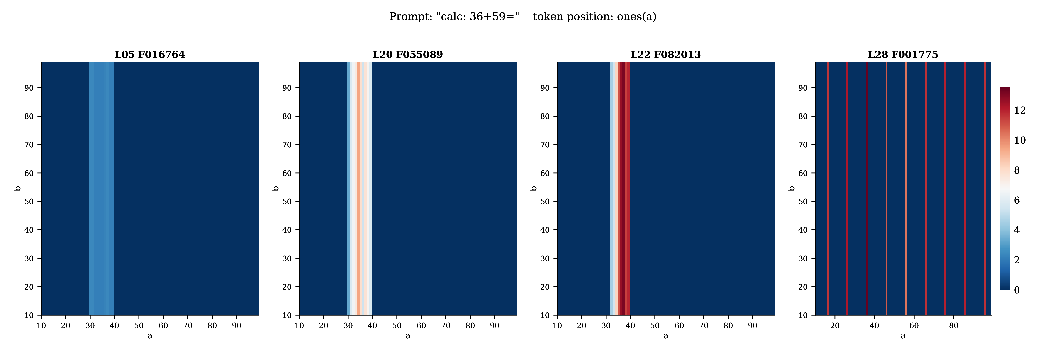
\includegraphics[width=\textwidth]{Pages/Figures/combined_ones(a)_filtered.pdf}
  \vspace{0.6em}
  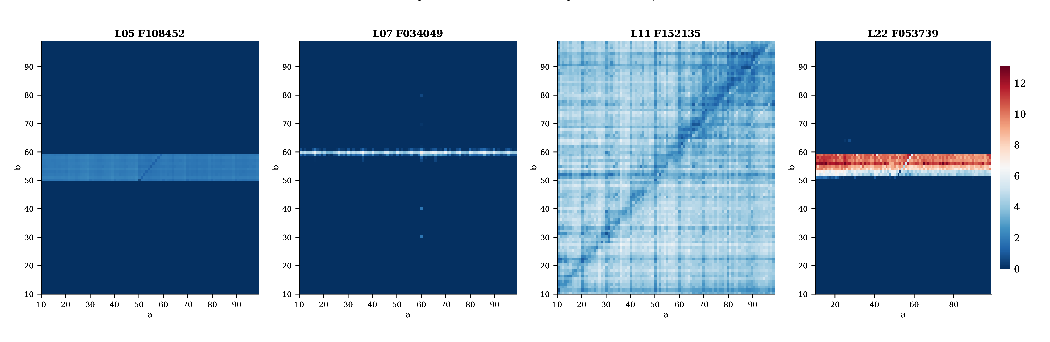
\includegraphics[width=\textwidth]{Pages/Figures/combined_ones(b)_filtered.pdf}
  \vspace{0.6em}
  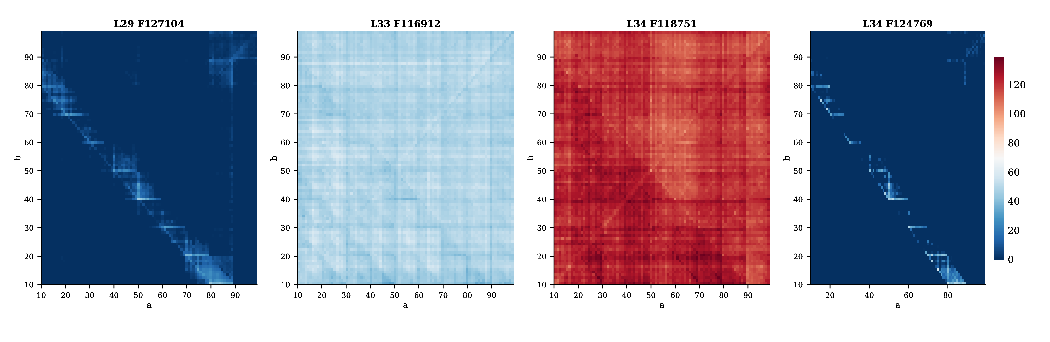
\includegraphics[width=\textwidth]{Pages/Figures/combined_=_filtered.pdf}
  \caption{Operand matrices at the two digit positions and the delimiter.}
  \label{fig:operand-pos-scan}
\end{figure}

\subsection{Full Addition Grid Accuracy and Exemplar}
\label{subsec:addition-dataset}

We use the full two-digit operand grid for feature discovery and one focus
prompt for attribution.

\begin{table}[ht!]
  \centering
  \small
  \caption{Prompt collections used in the addition reproduction.}
  \label{tab:addition-dataset}
  \begin{tabular}{@{}llrl@{}}
    \toprule
    Split & Template & $N$ & Purpose \\
    \midrule
    Operand grid
      & \promptinline{calc:~$a$+$b$=~}
      & $10{,}000$
      & Feature activation scan over $a,b \in \{0,\ldots,99\}$ \\
    Focus prompt
      & \promptinline{calc:~36+59=~}
      & $1$
      & Primary attribution graph with answer \promptinline{95} \\
    \bottomrule
  \end{tabular}
\end{table}

The grid covers all $100$ ones-digit combinations.  The focus prompt matches
the case used by \citet{lindsey2025biology}, so the same digit-pair hypothesis
can be tested across models.

\subsection{Teacher-Forced Accuracy Scan}
\label{subsec:accuracy-scan}

Before reading a circuit, we check that Qwen3-4B solves the task.  For each
$a,b \in \{0,\ldots,99\}$, we measure teacher-forced confidence at each answer
position.  If $\mathbf{y}^*(a,b)=(y^*_0,y^*_1,\ldots)$ is the correct answer
token sequence, then

\begin{equation}
  P_k(a,b)
  = P\!\left(
      y_k = y^*_k \;\middle|\;
      y_0 = y^*_0,\ldots,y_{k-1}=y^*_{k-1},\;
      \mathbf{x}(a,b)
    \right),
  \label{eq:teacher-forced}
\end{equation}

where $\mathbf{x}(a,b)$ is the prompt.  Teacher forcing removes uncertainty from
earlier generation errors and isolates the residual difficulty at position $k$.

Figure~\ref{fig:positional-cascade} shows a sharp cascade.  At $k=0$, the model
must infer the first output token from the operands alone, and the grid mean is
$\mu_0=0.233$.  Once this token is forced, confidence rises to $\mu_1=0.943$.
After the second token, it reaches $\mu_2=0.988$.  The hard step is the first
generated digit.  The $k=0$ panel is not smooth in operand magnitude.  It
repeats every ten cells, aligned with $(a \bmod 10,b \bmod 10)$.

\begin{figure}[ht!]
  \centering
  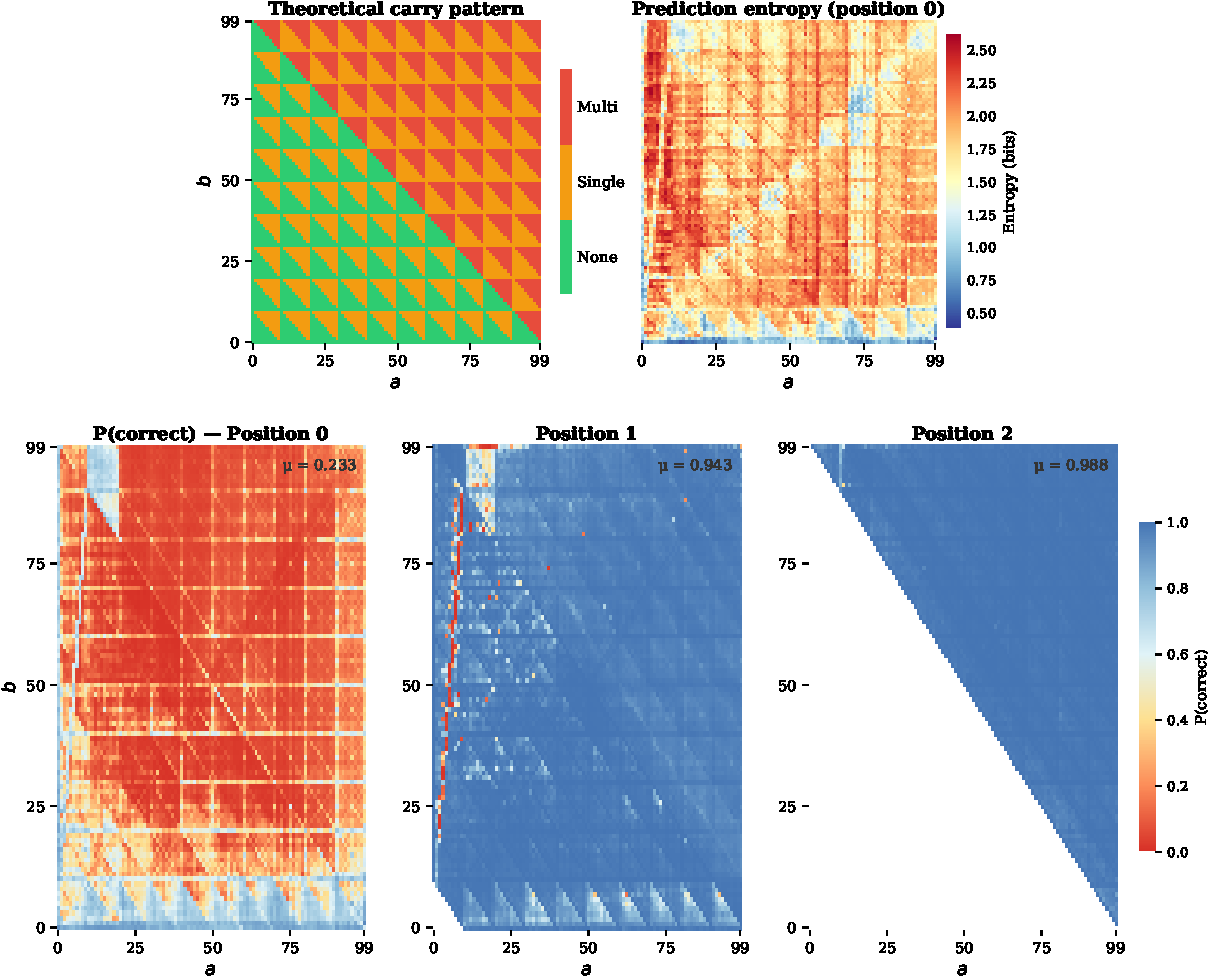
\includegraphics[width=\textwidth]{Pages/Figures/positional_cascade.pdf}
  \caption{Teacher-forced confidence over the full addition grid.}
  \label{fig:positional-cascade}
\end{figure}

\paragraph{Entropy and carry-class analysis.}
Prediction entropy and carry class give the same negative evidence.  Entropy is
highest near carry boundaries and larger sums, but confidence does not decrease
monotonically with carry count.  The period-10 digit-pair grid is the stronger
axis.

\paragraph{Addition circuit interpretation.}
In Qwen3-4B, the addition circuit reproduces the main signature reported for
Claude~3.5 Haiku.  The model reads each operand at its digit position, then recombines the two
residues at the delimiter through joint-modular and sum-sensitive features.  The first answer token carries most of the difficulty,
and its confidence is organised by ones-digit pairs.  These results support a
lookup-like account of this scanned \promptinline{calc:} format and two-digit
grid.  The evidence does not support a sequential carry-propagation account for
this specific setting.

\clearpage

\section{Multilingual Antonym Circuit Reproduction in Qwen3-4B}

\citet{lindsey2025biology} report that antonym completion in Claude~3.5 Haiku
separates the semantic operation, the operand concept, and the output language.
We treat this as a hypothesis rather than as a recipe.  The paper gives the
conceptual decomposition, while our experiment must define the Qwen prompts,
feature sets, layer ranges, and interventions explicitly.

We test whether the same separation appears in Qwen3-4B.  If operation and
operand features are language neutral, features identified from English should
still move French and Chinese outputs.  If output language is a separate
component, changing only language features should move the answer into another
language while preserving the antonym relation.  The following interventions
test these claims with the same transcoder suppress-and-inject procedure.

\subsection{Contrastive Feature Set Construction}
\label{subsec:exclusive-features}

Each experiment defines a source condition and a target condition that differ
in one component.  At layer $\ell$, let $a_{\ell,k}^{\mathrm{src}}$ and
$a_{\ell,k}^{\mathrm{tgt}}$ be the activation of transcoder feature $k$ under
the two conditions.  Among the top-$K$ active features, we define
source-exclusive and target-exclusive sets as

\begin{equation}
  \mathcal{S}^\ell
    = \left\{k \in \mathcal{F}_{\mathrm{src}}^\ell
        \;\middle|\; a_{\ell,k}^{\mathrm{tgt}} < \rho\,a_{\ell,k}^{\mathrm{src}}\right\},
  \qquad
  \mathcal{I}^\ell
    = \left\{k \in \mathcal{F}_{\mathrm{tgt}}^\ell
        \;\middle|\; a_{\ell,k}^{\mathrm{src}} < \rho\,a_{\ell,k}^{\mathrm{tgt}}\right\}.
  \label{eq:exclusive-sets}
\end{equation}

We fix the threshold at $\rho=0.5$.  We leave a feature unchanged when it is
active at comparable strength in both conditions.

\subsection{Feature Suppression and Injection Protocol}
\label{subsec:multilingual-intervention}

At the chosen layer and token position, we project the pre-MLP hidden state
$\mathbf{h}^{\ell,p}$ through the transcoder encoder,

\begin{equation}
  \tilde{\mathbf{z}}^{\ell,p}
    = \mathrm{ReLU}\!\left(
        \mathbf{W}_{\mathrm{enc}}^{(\ell)}\mathbf{h}^{\ell,p}
        + \mathbf{b}_{\mathrm{enc}}^{(\ell)}
      \right).
  \label{eq:reenc}
\end{equation}

We suppress source-exclusive activations and inject target-exclusive activations
with strength $\gamma$,

\begin{equation}
  \tilde{z}^{\ell,p}_k \leftarrow 0,
  \quad k \in \mathcal{S}^\ell;
  \qquad
  \tilde{z}^{\ell,p}_k \leftarrow \tilde{z}^{\ell,p}_k + \gamma v_k,
  \quad k \in \mathcal{I}^\ell,
  \label{eq:suppress-inject}
\end{equation}

where $v_k=a_{\ell,k}^{\mathrm{tgt}}$.  We decode the modified feature vector
back to residual space,

\begin{equation}
  \tilde{\mathbf{o}}^{\ell,p}
    = \mathbf{W}_{\mathrm{dec}}^{(\ell)}\tilde{\mathbf{z}}^{\ell,p}
      + \mathbf{b}_{\mathrm{dec}}^{(\ell)},
  \label{eq:decode-multi}
\end{equation}

then replace the standard MLP output at that site.  We monitor the next-token
probability

\begin{equation}
  \pi_t(\gamma)
    = \bigl[\mathrm{softmax}(\mathrm{logits}_T)\bigr]_t.
  \label{eq:pi-gamma}
\end{equation}

A successful component edit lowers the source token and raises the target token
as $\gamma$ increases.

\subsection{Operation, Operand, and Language Interventions}
\label{subsec:multilingual-experiments}

We use the layer ranges implied by the decomposition in
\citet{lindsey2025biology}, scaled to Qwen3-4B with $L=36$ layers,

\begin{equation}
  \mathcal{L}_{\mathrm{op}} = \{12,\ldots,23\},
  \qquad
  \mathcal{L}_{\mathrm{oper}} = \{0,\ldots,11\},
  \qquad
  \mathcal{L}_{\mathrm{lang}} = \{0,\ldots,6\}.
  \label{eq:layer-ranges}
\end{equation}

We do not fit these ranges to Qwen3-4B.  Success or failure therefore measures
how well the reported decomposition transfers.

\paragraph{Semantic-operation edit.}
We identify features using a source prompt that asks for the opposite of
``small'' and a target prompt that asks for a synonym of ``small''.  We select
features at the final token over $\mathcal{L}_{\mathrm{op}}$ and apply the edit
to English, French, and Chinese antonym prompts.  If operation features are
language neutral, the edit should move each language from an antonym toward a
synonym.

\paragraph{Operand-concept edit.}
We identify features using a source prompt that asks for the opposite of
``small'' and a target prompt that asks for the opposite of ``hot''.  We select
features at the operand divergence position over $\mathcal{L}_{\mathrm{oper}}$.
If operand features are language neutral, the edit should move the answer from
the antonym of \textit{small} toward the antonym of \textit{hot} in each
language.

\paragraph{Output-language edit.}
We identify features from source and target prompts that ask the same antonym
question in different languages.  We select features at the final token over
$\mathcal{L}_{\mathrm{lang}}$ for EN$\to$ZH, ZH$\to$FR, and FR$\to$EN.  If
language is a clean component, the edit should move probability into the target
language while preserving the antonym relation.

\subsection{Multilingual Intervention Outcomes}
\label{subsec:multilingual-results}

We use $K=15$ active features per layer and $\rho=0.5$.  We evaluate
probabilities on the token that actually follows the prompt, not on the token
obtained from a word in isolation.  This matters because quotation marks and
scripts change tokenisation.  In the French operand experiment, both
\textit{petit} and \textit{chaud} split into two subtokens.  We therefore apply
the intervention over the operand span, while the plot labels the intended
word.

\begin{figure}[htbp]
  \centering
  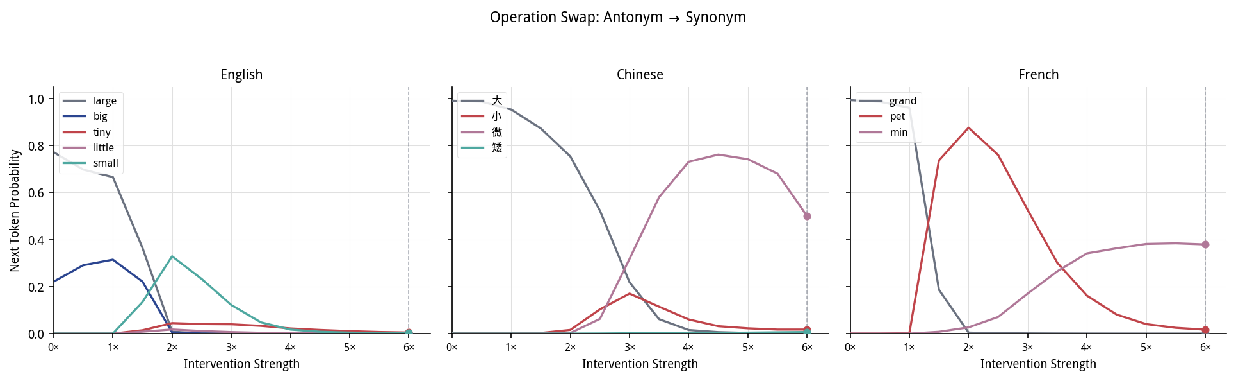
\includegraphics[width=0.96\textwidth]{Pages/Figures/op_swap.pdf}
  \caption{Operation edit across English, Chinese, and French.}
  \label{fig:multilingual-op-swap}
\end{figure}

\begin{figure}[htbp]
  \centering
  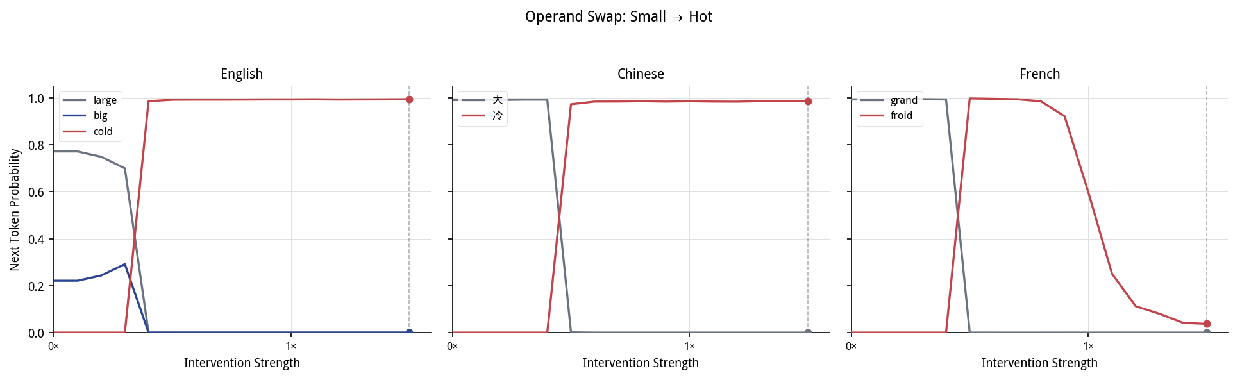
\includegraphics[width=0.96\textwidth]{Pages/Figures/operand_swap.pdf}
  \caption{Operand edit from \textit{small} to \textit{hot}.}
  \label{fig:multilingual-operand-swap}
\end{figure}

\begin{figure}[htbp]
  \centering
  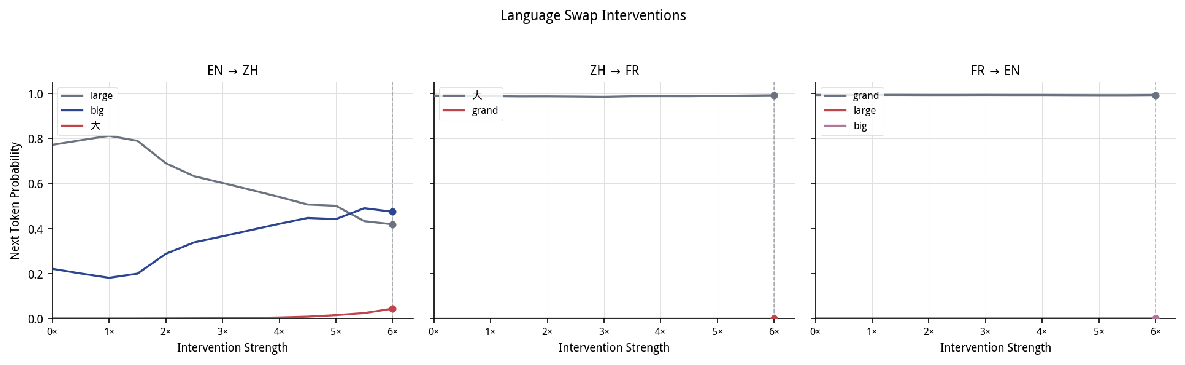
\includegraphics[width=0.96\textwidth]{Pages/Figures/lang_swap.pdf}
  \caption{Language edit between English, Chinese, and French.}
  \label{fig:multilingual-language-swap}
\end{figure}

\begin{table}[htbp]
  \centering
  \small
  \begin{tabular}{@{}llll@{}}
    \toprule
    Intervention & Case & Representative probability shift & Interpretation \\
    \midrule
    Operation & English & $P(\mathrm{big})$ from $0.68$ to $\approx 0$, $P(\mathrm{tiny})$ peaks at $0.35$ & partial crossover \\
    Operation & Chinese & $P(\text{d\`{a}})$ from $0.99$ to $\approx 0$, $P(\text{w\=ei})$ peaks at $0.75$ & crossover \\
    Operation & French  & $P(\textit{grand})$ from $0.43$ to $\approx 0$, $P(\textit{petit})$ peaks at $0.80$ & crossover \\
    \midrule
    Operand & English & $P(\mathrm{cold})$ from $2.1\!\times\!10^{-7}$ to $0.994$ & crossover \\
    Operand & Chinese & $P(\text{l\v{e}ng})$ from $1.5\!\times\!10^{-7}$ to $0.986$ & crossover \\
    Operand & French & $P(\textit{froid})$ from $1.5\!\times\!10^{-7}$ to $0.037$, target peak at $0.998$ & crossover \\
    \midrule
    Language & EN$\to$ZH & $P(\text{d\`{a}})$ from $2.3\!\times\!10^{-4}$ to $0.044$ & weak transfer \\
    Language & ZH$\to$FR & $P(\textit{grand})$ from $2.1\!\times\!10^{-7}$ to $2.3\!\times\!10^{-7}$ & no transfer \\
    Language & FR$\to$EN & $P(\textit{large})$ from $1.3\!\times\!10^{-5}$ to $9.5\!\times\!10^{-6}$ & no transfer \\
    \bottomrule
  \end{tabular}
  \caption{Multilingual intervention outcomes in Qwen3-4B.}
  \label{tab:multilingual-summary}
\end{table}

The operation intervention supports a shared semantic-operation component.  In
all three languages, antonym probability falls when we suppress antonym features
and inject synonym features.  Chinese and French show clear probability
transfer.  大 (d\`a) falls from $0.99$ to near zero while 微 (w\=ei) peaks at
$0.75$.  \textit{grand} falls while \textit{petit} peaks at $0.80$.  English is
weaker.  \textit{big} and \textit{large} are suppressed, but probability spreads
over several plausible synonyms, so \textit{tiny} peaks at $0.35$.  The common
signal is suppression of the antonym direction.  The weaker English target peak
comes from a broader output distribution.

The operand intervention is stronger.  The English-derived small-to-hot edit
moves the answer toward the antonym of \textit{hot} in English, Chinese, and
French.  English reaches $P(\mathrm{cold})=0.994$.  Chinese reaches
$P(\text{l\v{e}ng})=0.986$.  French is affected by subtokenisation, but the
target still crosses over.  The operand concept therefore transfers across the
three languages with little loss.

The language intervention does not reproduce a clean language component.  The
EN$\to$ZH edit weakly raises the Chinese answer token, but not enough to count
as an output-language swap.  ZH$\to$FR and FR$\to$EN produce no meaningful
transfer.  A supplementary edit that averages language features over the full
prompt suppresses the original answer, but still does not move mass to the
target-language token.  In Qwen3-4B, the selected early-layer MLP transcoder
features do not isolate output language.

\subsection{Attribution Graph Analysis}
\label{subsec:attr-graph}

Each attribution graph stores active transcoder features as nodes and
linearised influence weights as directed edges.  We read the graph by sorting
incoming edges to the target logit, then tracing the strongest upstream features
by layer, token position, and feature id.  The graph is a map of the measured
computation.

All graphs produced for this work are explorable at
\url{https://mechinterp-viz-94c364.uniofcam.dev/}.  Figure~\ref{fig:attr-graph-viz}
shows the attribution graph for \promptinline{calc:~36+59=}.  Nodes are arranged
by layer and token position.  Edge colour encodes sign.  Node size encodes
influence magnitude.  The dense mid-to-late layer region at the
\promptinline{=} token matches the lookup features identified above.

\begin{figure}[ht!]
  \centering
  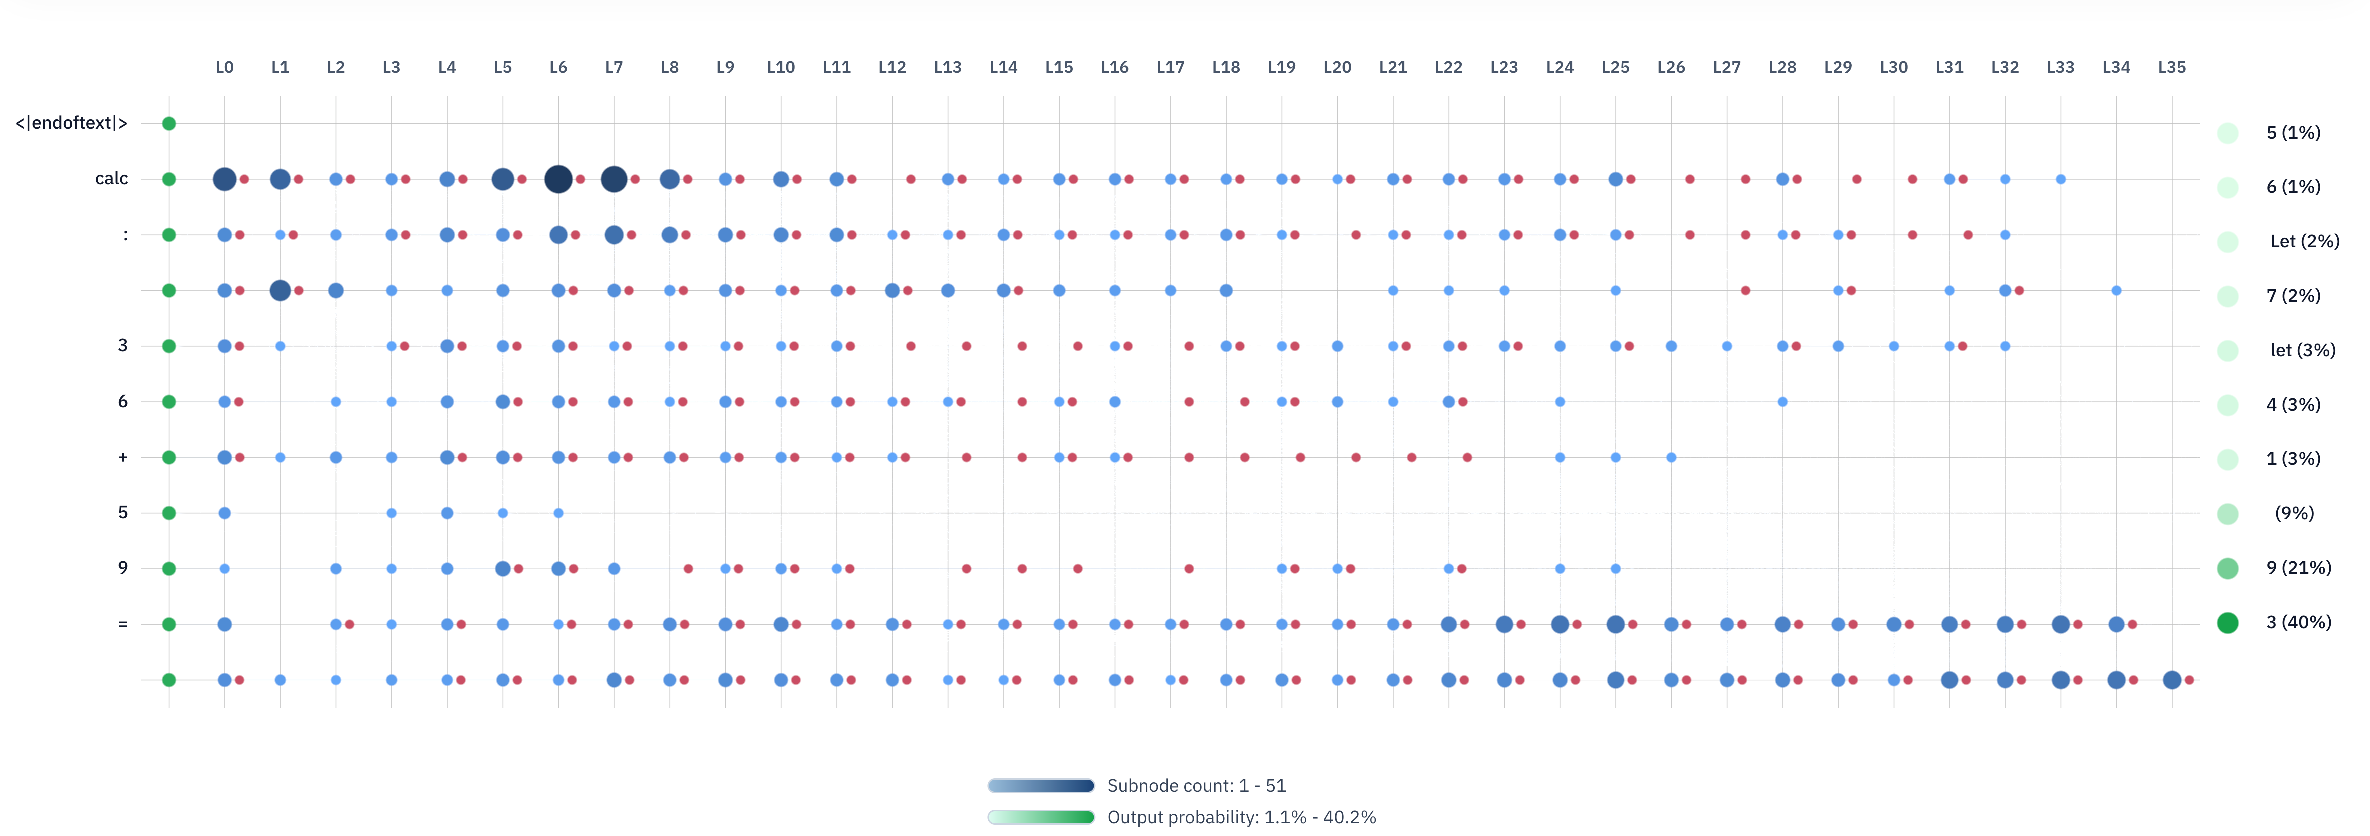
\includegraphics[width=\textwidth]{Pages/Figures/add_attr_graph_no_edges.pdf}
  \vspace{0.4em}
  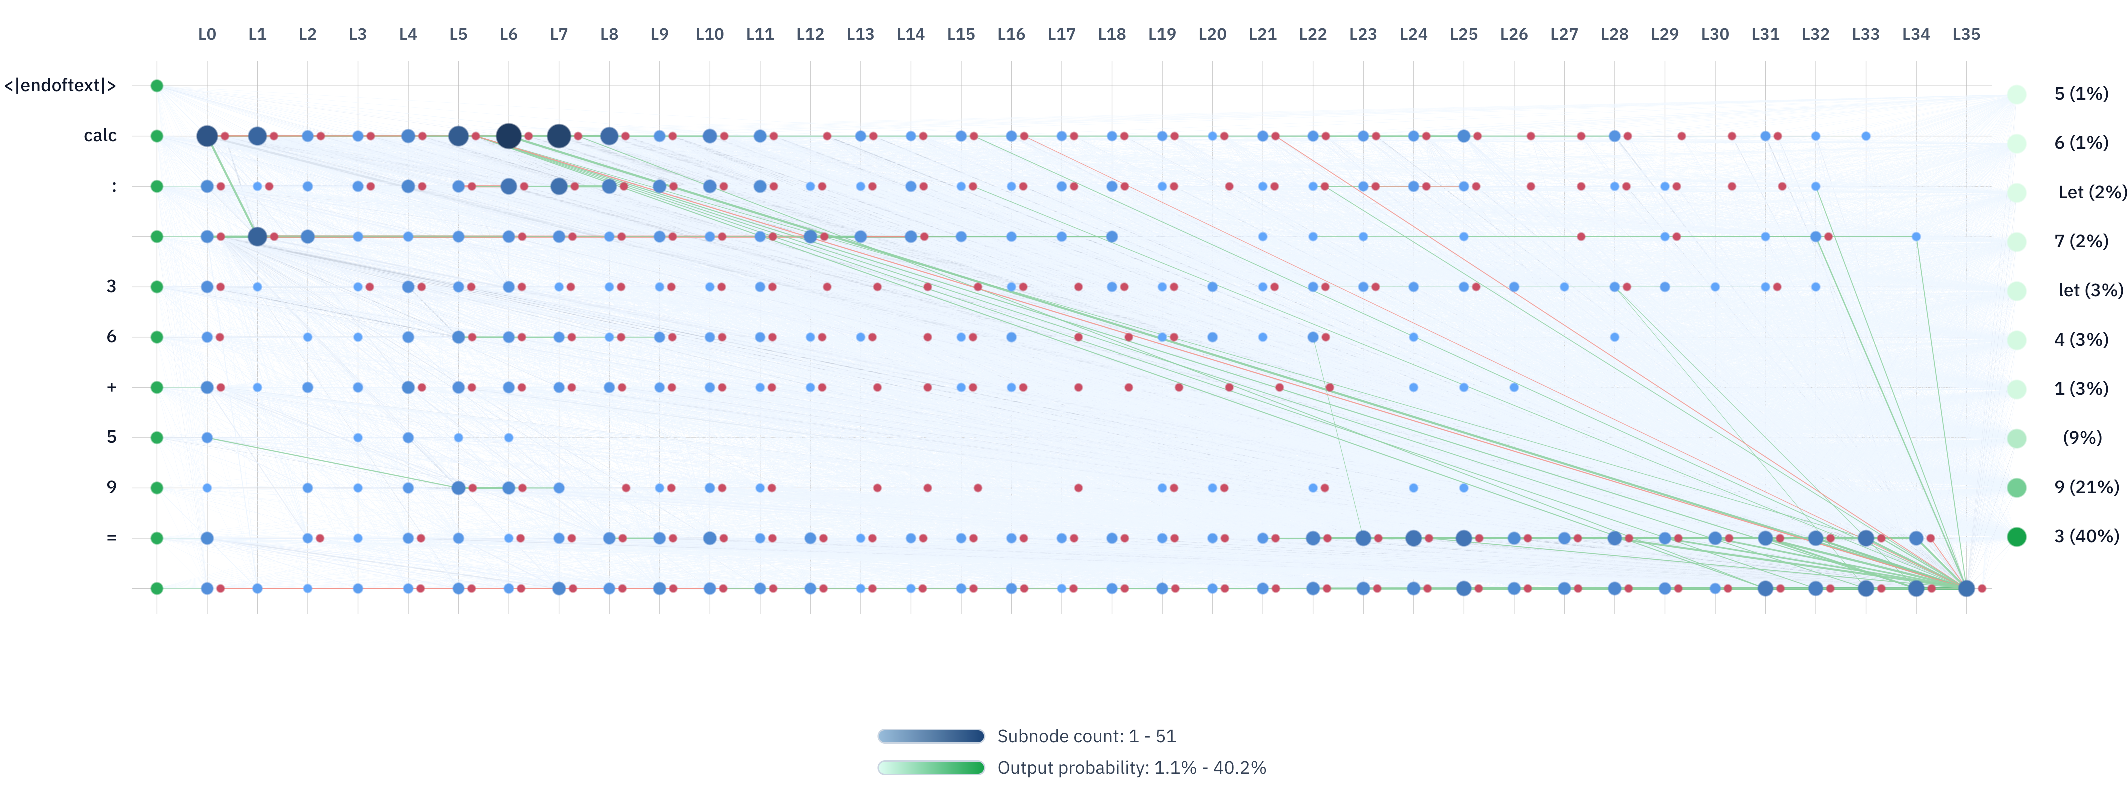
\includegraphics[width=\textwidth]{Pages/Figures/add_attr_graph_all_edges.pdf}
  \caption{Attribution graph for \promptinline{calc:~36+59=} at $N=0.75$. Upper panel shows attributed transcoder features at each layer and token position without edge routing. Lower panel shows the same graph with influence edges between features.}
  \label{fig:attr-graph-viz}
\end{figure}

\section{Reproduction Findings}
\label{sec:repro-conclusions}

For addition, Qwen3-4B recovers the digit-pair organisation reported for
Claude~3.5 Haiku.  The model reads the operands as separate decimal residues,
then combines these residues at the delimiter through modular and sum-sensitive
features.
Its uncertainty follows the lattice of ones digits more closely than the number
of carry steps.  On this template, the circuit is closer to a local lookup over
digit pairs than to written addition.

For multilingual antonyms, the separation is partial.  Operation and operand
edits transfer across English, French, and Chinese.  This suggests that Qwen3-4B
uses features for the semantic relation and for the operand concept that are not
bound to one language.  Output language behaves differently.  The same edit can
suppress the original answer without moving probability to the target-language
answer.  Meaning moves more cleanly than language form.

These results make the reproduction precise.  Some features transfer across
models and languages.  Others depend on tokenisation, layer range, or the exact
surface form of the task.  Reproduction therefore does not ask whether two
models contain the same circuit in every detail.  It asks which parts of the
computation remain stable when the model, tokeniser, and prompt surface change.
